\documentclass[10pt]{article}

% Lines beginning with the percent sign are comments
% This file has been commented to help you understand more about LaTeX

% DO NOT EDIT THE LINES BETWEEN THE TWO LONG HORIZONTAL LINES

%---------------------------------------------------------------------------------------------------------

% Packages add extra functionality.
\usepackage{
	times,
	graphicx,
	epstopdf,
	fancyhdr,
	amsfonts,
	amsthm,
	amsmath,
	algorithm,
	algorithmic,
	xspace,
	hyperref}
\usepackage[left=1in,top=1in,right=1in,bottom=1in]{geometry}
\usepackage{sect sty}	%For centering section headings
\usepackage{enumerate}	%Allows more labeling options for enumerate environments
\usepackage{epsfig}
\usepackage[space]{grffile}
\usepackage{booktabs}
\usepackage{amsmath}
\usepackage[super]{nth}
\usepackage{array}
\usepackage{tabularx}
\usepackage{multirow}
\usepackage{adjustbox}
\usepackage{longtable}


% This will set LaTeX to look for figures in the same directory as the .tex file
\graphicspath{.} % The dot means current directory.

\pagestyle{fancy}

\lhead{\YOURID}
\chead{\MyLang: Language Specification}
\rhead{\today}
\lfoot{CSCI 334: Principles of Programming Languages}
\cfoot{\thepage}
\rfoot{Spring 2022}

% Some commands for changing header and footer format
\renewcommand{\headrulewidth}{0.4pt}
\renewcommand{\headwidth}{\textwidth}
\renewcommand{\footrulewidth}{0.4pt}

% These let you use common environments
\newtheorem{claim}{Claim}
\newtheorem{definition}{Definition}
\newtheorem{theorem}{Theorem}
\newtheorem{lemma}{Lemma}
\newtheorem{observation}{Observation}
\newtheorem{question}{Question}

\setlength{\parindent}{0cm}
%---------------------------------------------------------------------------------------------------------

% DON'T CHANGE ANYTHING ABOVE HERE

% Edit below as instructed
\newcommand{\MyLang}{GeoDraw}	% Replace MyLang with your language name #
\newcommand{\PartnerOne}{Isabel Grondin}	% Replace PartnerOne with your name #
\newcommand{\PartnerTwo}{Meredith Wolf}	% Replace PartnerTwo with your partner's name #
\newcommand{\YOURID}{\PartnerOne{} + \PartnerTwo{}} % Remove \PartnerTwo if working alone.


\title{\MyLang: Language Specification}
\date{Spring 2022}
\author{\PartnerOne{} and \PartnerTwo{}} % Remove \PartnerTwo if working alone.

\begin{document}
\maketitle

\vspace{\baselineskip}	% Add some vertical space

% Refer to the lab handouts to determine what should go in each of these sections.  Each lab is additive.  So lab 8 should include everything you wrote in lab 7.  Lab 9 should include everything you wrote in lab 8, etc.

\section{Introduction}

GeoDraw is a language that lets you use basic math equations (lines, circles, parabolas, etc) to construct basic cartoon drawings. This is inspired by a project in high school that was designed to help us learn more about geometry through drawing cartoons using geometrical equations. It was difficult to find a graphing calculator online that made this particular project easy, for example, one where you have control over the colors of your lines. GeoDraw will be a be a fun educational tool to strengthen students knowledge of geometrical equations.
\\\\This language can also be viewed as a gentle introduction to computer graphics, which use much more complex mathematical equations, and to programming more generally. For that reason simplicity is an important part of our language design.


\section{Design Principles}

Our guiding principles are simplicity and readability. Since this language is targeted towards younger populations, who are most likely being introduced to programming, we want the language to be fairly intuitive. Furthermore, GeoDraw is a tool aiding students in learning graphing skills, and we do not want the complexity of the language to detract from that core objective.

\section{Example Programs}
All of the following examples can be run using typing "dotnet run example-X.geo" on the command line from the lang folder, with X representing the example number. Running the code will output a SVG file matching the name of the example in the lang folder. For example, example-1.geo with have an output file example-1.geo.svg. This SVG file can be opened and displayed in a browser. The output of the SVG files are displayed below.
\newpage
\textbf{Example 1: Diamond}

\begin{verbatim}
canvas(400, 400)
draw(y = abs((x - 200)), [], (74, 70, 166), 'simple')
draw(y = ((-1 * abs((x - 200))) + 400), [], (74, 70, 166), 'simple')
\end{verbatim}

\begin{center}
		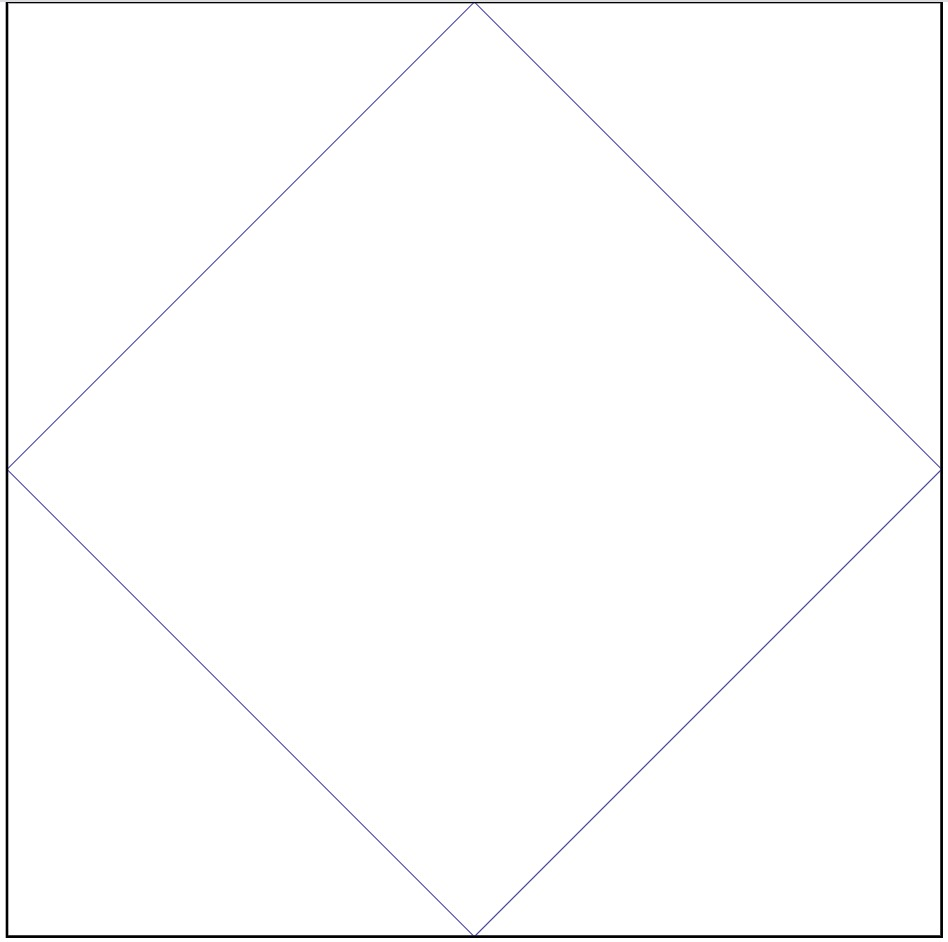
\includegraphics[scale=0.3]{images/example-1}
\end{center}

\textbf{Example 2: Smiley Face}

\begin{verbatim}
canvas(300, 300, (245, 212, 83))
draw(y = ((((x - 150) / 10) ^ 2) + 50), [x > 50, x < 250], (128, 96, 69), 'funky')
draw(y = ((-1 * (((x - 100) / 2.5) ^ 2)) + 250), [y > 200], (128, 96, 69), 'funky')
draw(y = ((-1 * (((x - 200) / 2.5) ^ 2)) + 250), [y > 200], (128, 96, 69), 'funky')
\end{verbatim}

\begin{center}
		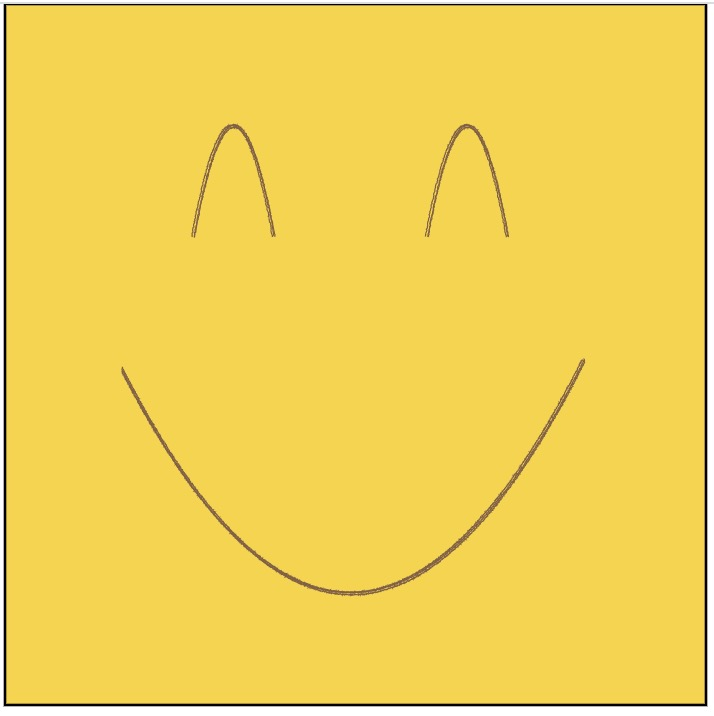
\includegraphics[scale=0.3]{images/example-2}
\end{center}

\textbf{Example 3: Ocean}
\begin{verbatim}
canvas(200, 200, (255,226,255))

# Create the waves
draw(y = (sin((x * .5)) * 10.5), [], (14, 255, 255), "thick")
draw(y = ((sin(((x * .5) + 5)) * 10.5) + 5), [], (65, 202, 202), "thick")
draw(y = ((sin(((x * .5) + 10)) * 10.5) + 10), [], (57, 183, 215), "thick")
draw(y = ((sin((x * .5)) * 10.5) + 15), [], (14, 255, 255), "thick")
draw(y = ((sin(((x * .5) + 5)) * 10.5) + 20), [], (65, 202, 202), "thick")
draw(y = ((sin(((x * .5) + 10)) * 10.5) + 20), [], (57, 183, 215), "thick")
draw(y = ((sin((x * .5)) * 10.5) + 25), [], (14, 255, 255), "thick")
draw(y = ((sin(((x * .25) + 5)) * 10.5) + 30), [], (65, 202, 202), "thick")
draw(y = ((sin(((x * .75) + 10)) * 10.5) + 35), [], (57, 183, 215), "thick")
draw(y = ((sin((x * .5)) * 10.5) + 40), [], (14, 255, 255), "thick")
draw(y = ((sin(((x * .75) + 5)) * 10.5) + 45), [], (65, 202, 202), "thick")
draw(y = ((sin(((x * .25) + 10)) * 10.5) + 50), [], (57, 183, 215), "thick")
draw(y = ((sin((x * .25)) * 10.5) + 50), [], (14, 255, 255), "thick")
draw(y = ((sin(((x * .75) + 5)) * 10.5) + 52), [], (65, 202, 202), "thick")
draw(y = ((sin(((x * .25) + 10)) * 10.5) + 54), [], (57, 183, 215), "thick")

# Create the moon
draw(y = (170 + sqrt (((30^2) - ((x - 170)^ 2)) )), [], (255, 255, 255), "thick")
draw(y = (170 - sqrt (((30^2) - ((x - 170)^ 2)) )), [], (255, 255, 255), "thick")
\end{verbatim}

\begin{center}
		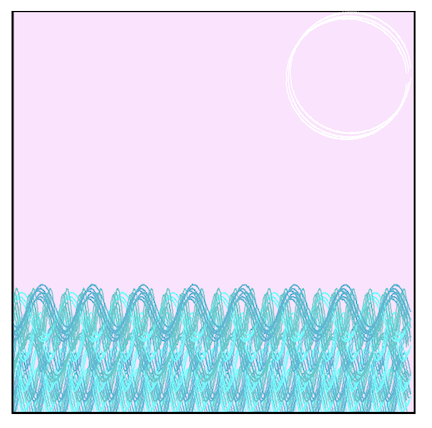
\includegraphics[scale=0.8]{images/example-3}
\end{center}


\section{Language Concepts}
The core concept a user needs to understand for GeoDraw is how to create an equation of the form $<$\texttt{Y}$><$\texttt{eq}$><$\texttt{Exp}$>$ to generate the desired line. An Expression,$<$\texttt{Exp}$>$ consists of the primitive data types $X$, real numbers, and operations. \texttt{Draw} is a combining form in our language that is made up of an equation, color, bounds, and brush style.

\newpage

\section{Syntax}

The syntax of the language is as follows:
\begin{itemize}
\item The overall program creates a drawing. A drawing is made up of:
\begin{itemize}
\item Canvas: The canvas is made up of the the height and the width of a canvas and a background color. The user does not need to specify a background color; the default color is white. The bottom left of the canvas is the point (0,0).
\item Draw: The draw function creates a line using the specified equation and bounds. Furthermore, the user must specify a color and a brush style for the line. We have three build in brush types: Simple, Funky, and Thick.
\end{itemize}
\end{itemize}

Here is the equivalent, formal definition of the grammar in Backus-Naur of GeoDraw (whitespace is ommitted for simplicity, but it can be added anywhere): \\\\
\ttfamily
\begin{tabular}{@{}ll@{}}
  $<\texttt{Sequence}>$ & $::=$ $<$\texttt{Canvas}$>$$<$\texttt{Expr}$>^{+}$ \\
  $<\texttt{Expr}>$ & $::=$ $<$Draw$>$ | <Sequence$>$ \\
	$<$Draw$>$ & $::=$ draw($<$Equation$>,<$Bound$>,<$Color$>,<$Brush$>$) \\
	$<$Canvas$>$ & $::=$ canvas$(<$CanvasNum$>,<$CanvasNum$>,<$Color$>) | $canvas$(<$CanvasNum$>,<$CanvasNum$>)$ \\
  $<$Equation$>$ & $::=$ $<$Y$><$Equality$><$Oper$>$ \\
  $<$Y$>$  & $::=$ Y | x \\
  $<$X$>$ & $::=$ X | x \\
  $<$Equality$>$ & $::=$  $< | = | >$ \\
  $<$Oper$>$  & $::=$ $<$Add$> | <$Sub$> | <$Div$> | <$Mult$> | <$X$> | <$Num$>$ \\
  $<$Sub$>$ & $ ::=$ $(<$Oper$>-<$Oper$>)$ \\
	$<$Div$>$ & $::=$ $(<$Oper$>/<$Oper$>)$ \\
	$<$Add$>$ & $::=$ $(<$Oper$> + <$Oper$> )$ \\
	$<$Mult$>$ & $::=$ $(<$Oper$> * <$Oper$> )$\\
	$<$Pow$>$ & $::=$ $(<$Oper$> \wedge <$Oper$> )$\\
	$<$Sin$>$ & $::=$ sin($<$Oper$>)$\\
	$<$Cos$>$ & $::=$ cos($<$Oper$>)$\\
	$<$Sqrt$>$ & $::=$ sqrt($<$Oper$>)$\\
	$<$Abs$>$ & $::=$ abs($<$Oper$>)$\\
  $<$Bound$>$ & $::=$ $[<$SingleBound$>] | [<$BoundList$>] | [$NoBounds$]$\\
	$<$SingleBound$>$ & $::=$ $<$Var$> <$Equality$> <$Num$>$ \\
	$<$BoundList$>$ & $::=$ $<$SingleBound$><$SingleBound$>^{+}$\\
	$<$Var$>$ & $::=$ $<$Xvar$> | <$Yvar$> | $VarError\\
	$<$Xvar$>$ & $::=$ X | x\\
	$<$Yvar$>$ & $::=$ Y| y\\
	$<$Color$>$ & $::=$ $(<$ColNum$>, <$ColNum$>, <$ColNum$>)$ \\
	$<$Brush$>$ & $::=$ Simple | Funky | Thick | Other\\
	$<$Num$>$ & $::=$ \textbf{R} \\
	$<$ColNum$>$ & $::=$ $0 \leq$ Int $\leq 255$\\
  $<$CanvasNum$>$ & $::=$ $0 \leq$ Int $\leq 600$\\
 \\
\end{tabular}
\rmfamily


\section{Semantics}
 We have the following primitive types: \texttt{x}, \texttt{y}, \texttt{float}, and equality symbols. Our main combining forms are \texttt{canvas}, \texttt{Color}, \texttt{Bound}, \texttt{Oper}, \texttt{Equation}, and \texttt{draw}. The first call of a program should always be \texttt{canvas}, and after that every call should be \texttt{draw}.

	\begin{center}
    \begin{longtable}{|p{20mm}|p{35mm}|p{15mm}|p{20mm}|p{55mm}|}
	  \hline
	  Syntax & Abstract Syntax & Type & Prec./Assoc. & Meaning \\
		\hline
	  $n$ & Num of float & float & N/A & Primitive value, represent using the f\# float type\\
	  \hline
	  $Y | y$ & Y & Y & N/A & Primitive value that we use when graphing equations\\
		\hline
	  $Y | y$ & varY & Var & N/A & Primitive value used inside of bounds\\
	  \hline
	  $X | x$ & X & Oper & N/A & Primitive value that we use when graphing equations \\
		\hline
	  $X | x$ & varX & Var & N/A & Primitive value used inside of bounds \\
		\hline
		$<$ & Less & Equality & N/A & Primitive value that we will use later when coloring shapes \\
		\hline
		$=$ & Equal & Equality & N/A & Primitive value that we will use later when coloring shapes \\
		\hline
		$>$ & Greater & Equality & N/A & Primitive value that we will use later when coloring shapes \\
		\hline
		$(o1 + o2)$ & Add of Oper * Oper & Oper & Unambiguous (parens) & Combining form that we use when calculating the line to graph \\
		\hline
		$(o1 - o2)$ & Sub of Oper * Oper & Oper & Unambiguous (parens) & Combining form that we use when calculating the line to graph \\
		\hline
		$(o1 / o2)$ & Div of Oper * Oper & Oper & Unambiguous (parens) & Combining form that we use when calculating the line to graph \\
		\hline
		$(o1 * o2)$ & Mult of Oper * Oper & Oper & Unambiguous (parens) & Combining form that we use when calculating the line to graph \\
		\hline
		$(o1 \wedge o2)$ & Pow of Oper $\wedge$ Oper & Oper & Unambiguous (parens) & Combining form that we use when calculating the line to graph \\
		\hline
		$ \sin o1$ & Sin of Oper & Oper & Unambiguous (parens) & Combining form that we use when calculating the line to graph \\
		\hline
		$ \cos o1$ & Cos of Oper & Oper & Unambiguous (parens) & Combining form that we use when calculating the line to graph \\
		\hline
		\text{sqrt} $o1$ & Sqrt of Oper & Oper & Unambiguous (parens) & Combining form that we use when calculating the line to graph \\
		\hline
		$ \text{abs } o1$ & Abs of Oper & Oper & Unambiguous (parens) & Combining form that we use when calculating the line to graph \\
		\hline
		$y = o$ & Equation of Y * Equality * Oper & Equation & N/A & Combining form that gives an equation for a line or curve to graph \\
		\hline
		$x < n \mid x > n \mid y < n \mid y > n$ & SingleBound of Var * Equality * float & Bound & N/A & Restricts the region that a line is graphed on \\
		\hline
		 (n, n, n) & Color of float list & Color & N/A & Represents a color in RGB format \\
		 \hline
 		 ‘simple’ $\mid$ ‘funky’ $\mid$ ‘thick’ $\mid$ ‘sparse’ $\mid$ ‘wide’ $\mid$ s & Simple $\mid$ Funky $\mid$ Thick $\mid$ Sparse $\mid$ Wide $\mid$ Other of s &
		 Brush & N/A & Brush type to use when drawing a specific line. Simple is a single line, while Funky and Thick are preprogrammed \\
		 \hline
 		 draw(e, [bounds], c, brush) & Draw of Equation * Bound * Color * Brush &
		 Expr & N/A & Combining form to draw a line. Contains the equation for the line, bounds within which the line should be drawn, color for the line, and brush type for the line. \\
		 \hline
 		 canvas$(n, n)$ $\mid$ canvas$(n, n, c)$ & Canvas of float * float * Color &
		 Expr & N/A & Sets the canvas on which the user will be drawing, and sets its background color optionally. This line MUST be called as the first line in a program, and must not be called again. \\
		 \hline
 		 gridlines$(i)$ & Gridline of int & Expr & N/A & Adds a grid to the canvas at the specified interval i. i must be a positive integer \\
		 \hline
 		 brush s = [points] & Assignment of string * (float*float) list & Expr & N/A & Creates a custom brush with the specified points, where \emph{points} is a list of float 2-tuples where x and y are on the interval $[0, 5]$\\
		 \hline
 		 \# s & N/A & N/A & N/A & Everything on a line after the ‘\#’ is a comment and will not be parsed. Comments cannot have additional pound signs within them.\\
	  \hline
	\end{longtable}
	\end{center}

	The user must first create a canvas by inputting a height, width and an optional background color. Drawings will end at the sides of the canvas unless bounds are specified. Drawings are the main elements in the language. They are a combination of an equation, its bounds, a color, and a brush style. Equations must have the y variable on the left, an $=$, followed by a mathematical expression. Bounds denote the limits of the equation for x, y, or both. Mathematical expressions combine our operations, real numbers, and the x variable. Brush styles consist of a string, which indicates a brush strokes type we have created. \\\\

	Our programs does not read any input. The user must input a program as a file. The output of evaluating the program is a drawing consisting of the lines specified in the program. This is in the form of an SVG file. \\\\

	\textbf{Hierarchy Drawing:}\\
	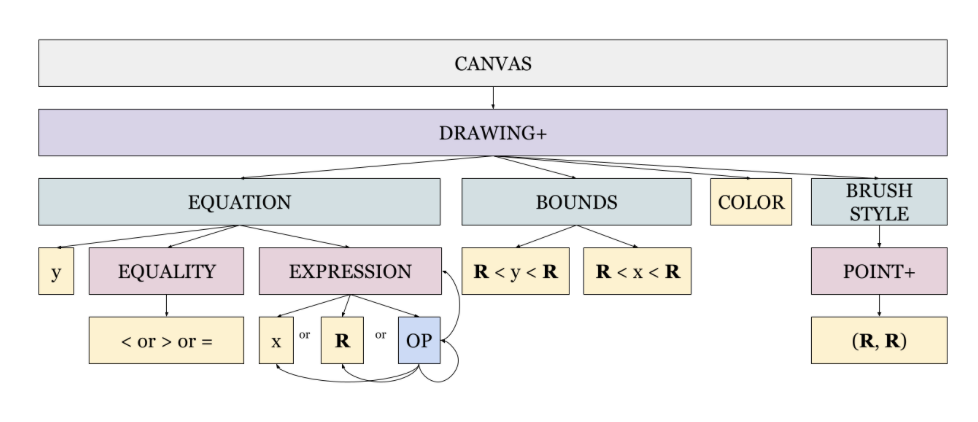
\includegraphics[scale=0.36]{images/hierarchyDrawing} \\
	\newpage
	\textbf{AST for Example 1:}\\
	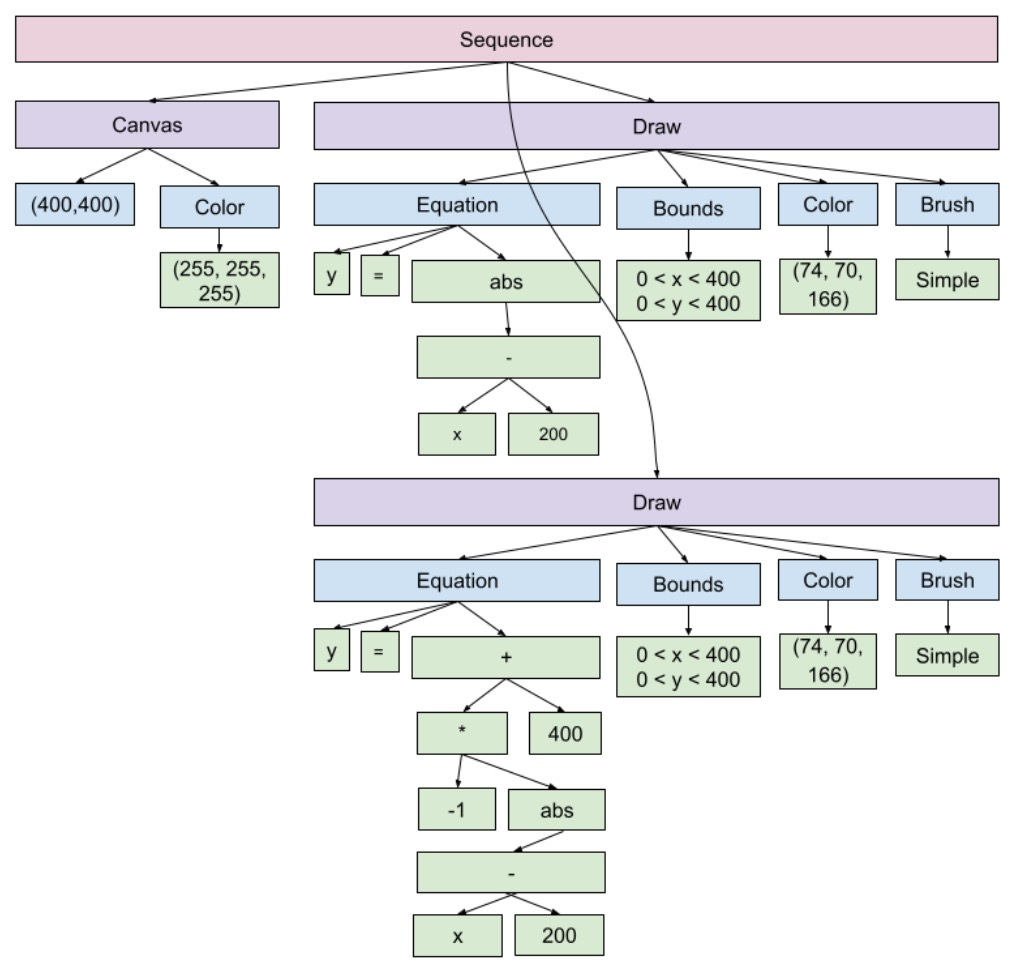
\includegraphics[scale=0.4]{images/astExample1.jpeg}


\section{Remaining Work:} We would like to implement a custom brush feature, that allows the user to design a brush by entering a list of points and store this to use throughout a program. We are also interested in making our selection of available brushes more robust. \\

Right now, all equations must be functions with x as the independent variable and y as the dependent variable. We would like to add functionality to allow x on the left side of the equation to improve user experience and allow for vertical lines. As a stretch goal, we would like to implement inequality shading for our equations.


% DO NOT DELETE ANYTHING BELOW THIS LINE
\end{document}
